\documentclass[border=15pt, multi, tikz]{standalone}


\usepackage{tikz}
\usetikzlibrary{quotes,arrows.meta}
\usetikzlibrary{positioning}
\def\edgecolor{rgb:blue,4;red,1;green,4;black,3}
\newcommand{\midarrow}{\tikz \draw[-Stealth,line width =0.8mm,draw=\edgecolor] (-0.3,0) -- ++(0.3,0);}
\usepackage{Box}
\usepackage{RightBandedBox}

\def\ConvColor{rgb:blue,5;green,2.5;white,5}
\def\ConvReluColor{rgb:blue,5;green,5;white,5}
\def\PoolColor{rgb:red,1;black,0.3}
\def\DcnvColor{rgb:blue,5;green,2.5;white,5}
\def\UnpoolColor{rgb:yellow,5;red,2.5;white,5}
\def\SoftmaxColor{rgb:magenta,5;black,7}

\usetikzlibrary{3d} %for including external image 

\definecolor{Auburn}{HTML}{9E2A2B}

\tikzset{hencoder/.style={
  minimum width=1cm,
  minimum height=0.7cm,
  rectangle,
  rounded corners=3pt,
  fill=Auburn,
  text=white,
  line width=0.5mm,
  draw=Auburn!50}}

\begin{document}

\begin{tikzpicture}
\tikzstyle{connection}=[ultra thick,every node/.style={sloped,allow upside down},draw=\edgecolor,opacity=0.7]
%%%%%%%%%%%%%%%%%%%%%%%%%%%%%%%%%%%%%%%%%%%%%%%%%%%%%%%%%%%%%%%%%%%%%%%%%%%%%%%%%%%%%%%%
%% Draw Layer Blocks
%%%%%%%%%%%%%%%%%%%%%%%%%%%%%%%%%%%%%%%%%%%%%%%%%%%%%%%%%%%%%%%%%%%%%%%%%%%%%%%%%%%%%%%%
%%%%%%%%%%   
\node (input) at (0,3.5,0) {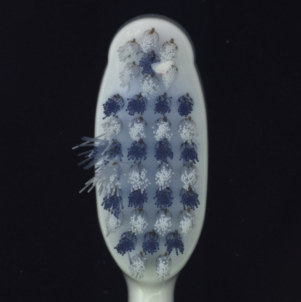
\includegraphics[width=3cm,height=3cm]{img/sub-img/toothbrush-defective.png}};
\node (labelinput) at (0,1.5,0) {input};

\node[hencoder] (euclide) at (4,3.5,0) {Distance euclidienne};

\node (output) at (8,3.5,0) {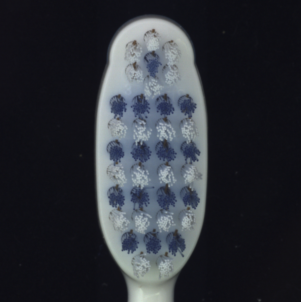
\includegraphics[width=3cm,height=3cm]{img/sub-img/toothbrush.png}};
\node (labeloutput) at (8,1.5,0) {output};

\node (heatmap) at (4,0,0) {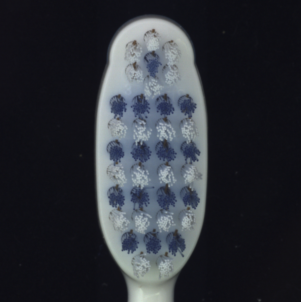
\includegraphics[width=3cm,height=3cm]{img/sub-img/toothbrush.png}};

%Connections
\path[->,>=stealth] (input.east) edge node [left] {} (euclide.west);
\path[->,>=stealth] (output.west) edge node [left] {} (euclide.east);
\path[->,>=stealth] (euclide.south) edge node [left] {} (heatmap.north);
\end{tikzpicture}
\end{document}\grid
